% CFP: https://discourse.llvm.org/t/cfp-llvm-hpc-workshop-at-sc-25/86391
% At least 5 two-column pages, excluding the bibliography and figures

% Submission: Aug 15, 2025
% Internal deadline: Aug 4, 2025

% Topics:
% 1) The LLVM IR generated by OpenMPIRBuilder can be easily optimized by OpenMPOpt pass (the old flang cannot do it)
% 2) The support of math functions for AMDGPU is done by MLIR code which is also used for GPU-specific optimization for other workloads.
% 3) We can reuse AMD downstream NO_LOOP mode which was written for OpenMP C for Fortran (in progress, but the tests show that it's beneficial)

% Detailed plan for #2 proposal:

% General issues:
% Terminology:
%   array descriptor vs dope vector?
% Default compiler:
%   AOMP Flang/upstream flang?
% Default GPU?
% Are we allowed to present some numbers from microbenchmarks? (i.e. very small code snippets used only for illustration of the problem)

% 1) Handling of descriptors of Fortran pointers and allocatable arrays (The code with allocatable arrays requires more resources in comparison to stack arrays)
%  -> Fortran differences between static and dynamic arrays vs C:
%     a) static -> the size is known in compilation time
%     b) dynamic -> the size and shape is unknown in compilation time
%     c) allocate vs malloc in C
%        * allocate -> defines the shape and size of the allocated array. The information about size/shape and the beginning of allocated memory is stored in array descriptor.
%        * malloc -> allocates N consecutive bytes and it returns address of the first byte
%  -> MLIR(HLFIR + FIR)+LLVM IR code analysis of simple operation a[i] = 5 for static and dynamic arrays for code:
%  !$omp target teams distribute parallel do map(tofrom: x)
%  do i = 1, 255
%    x(i) = a(i) + b(i)
%   end do
%     a) host side + mapping
%     b) GPU side
%  -> Comparison of required resources for exemplary kernels: SGPRS/VGPRS for different optimization levels (are we allowed?)

% 2) Problems related to temporary arrays (i.e.: iaVS = [ iV, jV, kV ] + iaS ) and option -fstack-arrays as remedy.
%  -> Flang default handling of temporary arrays (heap allocation)
%  -> Example of usage of temporary array inside GPU code
%  -> Explanation how heap array is handled inside GPU kernel (slow malloc call)
%  -> Explanation of option -fstack-arrays
%  -> Advantages and disadvantages of option -fstack-arrays (Possible stack overflow vs faster GPU kernels)
%  -> Comparison of execution times for kernel with temporary array with and without -fstack-array (are we allowed?)

%% Lower priority, only as space and time permits:
%% 3) The Fortran runtime calls which can involuntarily appear in the GPU code
%% -> Description of Fortran runtime
%%  -> Examples of Fortran code where Fortran runtime is used
%%  -> Consequences of Fortran runtime call inside GPU kernel (are we allowed to present some execution times?)
\documentclass[acmtog,natbib=false]{acmart}
\AtBeginDocument{\providecommand\BibTeX{{Bib\TeX}}}

\RequirePackage[
datamodel=acmdatamodel,
style=acmnumeric, % use style=acmauthoryear for publications that require it
]{biblatex}
\addbibresource{references.bib}

\usepackage[T1]{fontenc}
\usepackage{listings}
\usepackage{minted}
\usepackage{xspace}
\usepackage[printonlyused]{acronym}

% Enabling the next line pushes all figures to the end the paper.
% Michael will occasionally do that to check the page count.
%\usepackage[nomarkers,figuresonly]{endfloat}

%% Rights management information.  This information is sent to you
%% when you complete the rights form.  These commands have SAMPLE
%% values in them; it is your responsibility as an author to replace
%% the commands and values with those provided to you when you
%% complete the rights form.
\setcopyright{acmlicensed}
\copyrightyear{2025}
\acmYear{2025}
\acmDOI{XXXXXXX.XXXXXXX}

%%
%% Submission ID.
%% Use this when submitting an article to a sponsored event. You'll
%% receive a unique submission ID from the organizers
%% of the event, and this ID should be used as the parameter to this command.
\acmSubmissionID{tbd}

%% the listings
\lstset{
  captionpos=b,
}
\setminted{
  escapeinside=||,
  fontsize=\small,
  baselinestretch=0.8,
  linenos,
  numbersep=0.5em,
  xleftmargin=1em
}

%% useful macros
\newcommand{\todo}[1]{\textcolor{red}{#1}}
\newcommand{\code}[1]{\texttt{#1}\xspace}
\newcommand{\registered}[0]{\textsuperscript{\textregistered}\xspace}
\newcommand{\trademark}[0]{\texttrademark\xspace}

\begin{document}
\title{Implementing OpenMP\registered Offload Support in LLVM Flang}

\author{Dominik Adamski}
\email{dominik.adamski@amd.com}
\orcid{}
\affiliation{%
  \institution{Advanced Micro Devices}
  \city{Lodz}
  \state{lodzkie }
  \country{Poland}
}

\author{Akash Banerjee}
\email{akash.banerjee@amd.com}
\orcid{}
\affiliation{%
  \institution{Advanced Micro Devices}
  \city{Milton Keynes}
  \state{England}
  \country{UK}
}

\author{Kareem Ergawy}
\email{kareem.ergawy@amd.com}
\orcid{0009-0002-6326-8664}
\affiliation{%
  \institution{Advanced Micro Devices GmbH}
  \city{Munich}
  \state{BY}
  \country{Germany}
}

\author{Andrew Gozillon}
\email{andrew.gozillon@amd.com}
\orcid{0000-0001-7558-7166}
\affiliation{%
  \institution{Advanced Micro Devices AB}
  \city{Malmo}
  \state{Skåne County}
  \country{Sweden}
}

\author{Michael Klemm}
\email{michael.klemm@amd.com}
\orcid{0000-0002-8634-4634}
\affiliation{%
  \institution{Advanced Micro Devices GmbH}
  \city{Munich}
  \state{BY}
  \country{Germany}
}

\author{Jan Leyonberg}
\email{jan.leyonberg@amd.com}
\orcid{}
\affiliation{%
  \institution{Advanced Micro Devices}
  \city{Toronto}
  \state{ON}
  \country{Canada}
}

\author{Dan Palermo}
\email{dan.palermo@amd.com}
\orcid{0009-0005-7205-2250}
\affiliation{%
  \institution{Advanced Micro Devices}
  \city{Austin}
  \state{TX}
  \country{USA}
}

\renewcommand{\shortauthors}{Adamski et al.}

\begin{abstract}
\todo{Michael: write the abstract.}
\todo{Lorem ipsum dolor sit amet, consectetur adipisicing elit, sed do eiusmod
tempor incididunt ut labore et dolore magna aliqua. Ut enim ad minim veniam,
quis nostrud exercitation ullamco laboris nisi ut aliquip ex ea commodo
consequat. Duis aute irure dolor in reprehenderit in voluptate velit esse
cillum dolore eu fugiat nulla pariatur. Excepteur sint occaecat cupidatat non
proident, sunt in culpa qui officia deserunt mollit anim id est laborum.
Lorem ipsum dolor sit amet, consectetur adipisicing elit, sed do eiusmod
tempor incididunt ut labore et dolore magna aliqua. Ut enim ad minim veniam,
quis nostrud exercitation ullamco laboris nisi ut aliquip ex ea commodo
consequat. Duis aute irure dolor in reprehenderit in voluptate velit esse
cillum dolore eu fugiat nulla pariatur. Excepteur sint occaecat cupidatat non
proident, sunt in culpa qui officia deserunt mollit anim id est laborum.}
\end{abstract}

%% generate via: https://dl.acm.org/ccs
\begin{CCSXML}
<ccs2012>
   <concept>
       <concept_id>10011007.10011006.10011041</concept_id>
       <concept_desc>Software and its engineering~Compilers</concept_desc>
       <concept_significance>500</concept_significance>
       </concept>
   <concept>
       <concept_id>10010147.10010169.10010175</concept_id>
       <concept_desc>Computing methodologies~Parallel programming languages</concept_desc>
       <concept_significance>500</concept_significance>
       </concept>
   <concept>
       <concept_id>10010520.10010521.10010542.10010546</concept_id>
       <concept_desc>Computer systems organization~Heterogeneous (hybrid) systems</concept_desc>
       <concept_significance>500</concept_significance>
       </concept>
 </ccs2012>
\end{CCSXML}
\ccsdesc[500]{Software and its engineering~Compilers}
\ccsdesc[500]{Computing methodologies~Parallel programming languages}
\ccsdesc[500]{Computer systems organization~Heterogeneous (hybrid) systems}

\keywords{LLVM, Flang, OpenMP, GPU, Accelerators}

\received{by 15 August 2025}
\received[revised]{TBD}
\received[accepted]{TBD}

\maketitle

%%%%%%%%%%%%%%%%%%%%%%%%%%%%%%%%%%%%%%%%%%%%%%%%%%%%%%%%%%%%%%%%%%%%%%%%%%%%%%%%%%%%%%%%%%%%%%%%%%%%%%%%%%%%
%%%%%%%%%%%%%%%%%%%%%%%%%%%%%%%%%%%%%%%%%%%%%%%%%%%%%%%%%%%%%%%%%%%%%%%%%%%%%%%%%%%%%%%%%%%%%%%%%%%%%%%%%%%%

\section{Introduction}
\label{sec:Introduction}
\todo{Michael: Write the introduction part}

\todo{
\begin{itemize}
\item Fortran standard supported by Flang
\item OpenMP versions supported by Flang
\item Implementations of features driven by request and usefulness, not by historic order.
\end{itemize}
}

%%%%%%%%%%%%%%%%%%%%%%%%%%%%%%%%%%%%%%%%%%%%%%%%%%%%%%%%%%%%%%%%%%%%%%%%%%%%%%%%%%%%%%%%%%%%%%%%%%%%%%%%%%%%
%%%%%%%%%%%%%%%%%%%%%%%%%%%%%%%%%%%%%%%%%%%%%%%%%%%%%%%%%%%%%%%%%%%%%%%%%%%%%%%%%%%%%%%%%%%%%%%%%%%%%%%%%%%%

\section{LLVM Flang Compiler}
\label{sec:LLVMFlangCompiler}

At the time of writing this paper, the AMD Fortran compiler toolchain is undergoing a transition.
AMD is actively working on developing the AMD Next-Gen Fortran compiler that will eventually replace the existing AMD Fortran Compiler for the AMD ROCm\trademark platform.
While the current Fortran compiler that ships with AMD ROCm\trademark package is based on the PGI\registered compiler code~\cite{Lara17,Pric17}, the AMD Next-Gen Fortran Compiler is based on the LLVM Flang compiler~\cite{LLVM25}.
AMD plans to make this the new production compiler that will ship with a future version of the AMD ROCm\trademark software stack.

\begin{figure}[t]
\centering
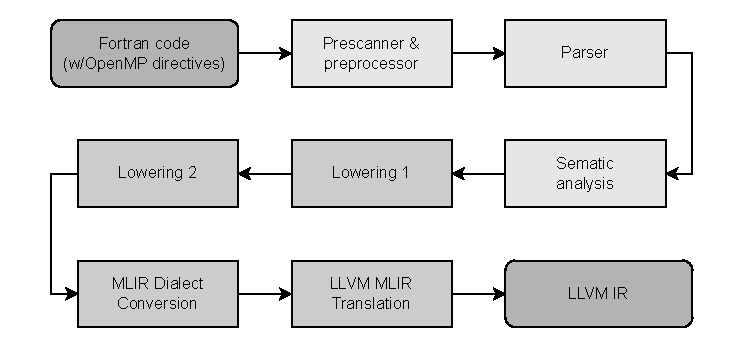
\includegraphics[width=\linewidth]{figures/flang_compiler_phases_overview.pdf}
\caption{Simplified overview of the compiler phases in the AMD Next-Gen Fortran Compiler front-end.\label{fig:FlangCompilerPhases}}
\end{figure}

\begin{listing}[t]
\inputminted{Fortran}{code/tgt_loop.f90}
\caption{Example Fortran code with \code{!\$omp target teams loop} construct and \code{map} clauses.}
\label{lst:FortranExample}
\end{listing}

\begin{listing}[t]
\inputminted{Fortran}{code/tgt_loop_cooked.f90}
\caption{Fortran code of Listing~\ref{lst:FortranExample} after preprocessing and prescanning.}
\label{lst:FortranExampleCooked}
\end{listing}

Figure~\ref{fig:FlangCompilerPhases} shows a simplified overview of the compiler pipeline of the LLVM Flang compiler frontend up to LLVM \ac{IR} generation.
The same stages are also used by the AMD Next-Gen Fortran Compiler front-end.
In the Prescanner \& Preprocessor stage, the lexical analysis and C-style processor produce a stream of characters of normalized Fortran source code. 
This code contains expanded preprocessor macros, included code resulting from \code{INCLUDE} statements. Unnecessary blank characters and comments are also removed in this stage (see Listing~\ref{lst:FortranExampleCooked}).
Compiler directives such as \code{!\$dir} and the OpenMP directives introduced with \code{!\$omp} remain in the stream of characters.
The parser and semantic analysis stages then construct a parse tree of the processed Fortran code and annotate it with semantic information (e.g., data types).
The parse tree contains all details about OpenMP directives, clauses, etc. as nodes in the tree.

\begin{listing}[t]
\inputminted{MLIR-lexer.py:MlirLexer -x}{code/tgt_loop_abridged.fir}
\caption{Abridged intermediate representation of the Fortran code in Listing~\ref{lst:FortranExample} with \ac{FIR} and OpenMP \ac{MLIR} dialects.}
\label{lst:FortranExampleFIR}
\end{listing}

The parse tree is then gradually lowered into different levels of intermediate representation, depending on the needs of the applied transformation and optimization passes.

First, the parse tree is transformed into the \ac{MLIR} \ac{HLFIR} and \ac{FIR} (see \ac{FIR} code in  Listing~\ref{lst:FortranExampleFIR}).
These intermediate representations provide entities that correspond to Fortran language elements.
\Ac{HLFIR} provides additional high-level information over \ac{FIR} about the specific features and semantics of Fortran (e.g., array operations that can be used to optimize Fortran array statements).
It also has additional information in the type system to represent Fortran attributes for (dummy) variables.

OpenMP directives and clauses are reflected in this intermediate representation via an additional \ac{MLIR} dialect that mixes with \ac{HLFIR} and \ac{FIR}.
Through these additional elements, the intermediate representation contains explicit information about  OpenMP directives and clauses in the code as well as their nesting structure.
For instance, \code{DO} loop nest is associated with the corresponding OpenMP \code{target teams loop} construct (see Listing~\ref{lst:FortranExampleFIR}).
Finally, the \ac{MLIR} code is transformed into regular LLVM \ac{IR} and is passed to the compiler back-end for target code generation.


\section{OpenMP Code Generation}
\label{sec:OpenMPCodeGen}

To generate code for device execution that adheres to the OpenMP semantics, the compiler has to perform these steps:

\begin{itemize}
\item identify implicitly and explicitly mapped variables for a \code{target} construct;
\item outline the \code{target} constructs into a separate function;
\item generate boilerplate code to invoke the outlined function and pass data-mapping information to it; and
\item link the individual object files with host and device code to produce the final executable.
\end{itemize}

We will provide an overview of the above steps in the remainder of this section.

\subsection{OpenMP Data Mapping Analysis}
\label{sec:OpenMPDataMappingAnalysis}

Each entry in a \code{map} clause is processed individually and generates an individual \code{map.info} operation. 
The information specified by an explicit \code{map} clause has all the information required to populate an \code{map.info} operation. 
The OpenMP \code{map type modifier} (\code{to} in Line~\ref{ln:SaxpyMapClause} in Listing~\ref{lst:FortranExampleFIR}) specified by the clause applies to each \code{map.info} generated, and is tracked by the operations \code{map\_clause} field. 
The provided variable names (symbols), allow the compiler to gather the base address, type and boundary data for the mapped data, populating the \code{var\_ptr} and \code{bounds} field of the operation. 
The \code{capture} field for explicitly mapped data is set to always be by reference for the moment.

In Listing~\ref{lst:FortranExample} it can be seen that there is variables referenced within the \code{target} region and not within a \code{map} clause. 
This information is still required on the device for the correct execution of the kernel, and it is up to the compiler to gather and implicitly generate \code{map.info} operations for these, in an action known as capturing. 
The OpenMP specification~\cite{OARB24} defines rules for how these variables should be handled by the compiler and runtime, which LLVM Flang adheres to. 

The capturing of variables occurs during the initial lowering of the \code{target} node, after all of its attached clauses have been processed; including the \code{map} clause. 
At this stage the compiler has knowledge of what symbols have already been mapped to device by the varying data movement clauses and can proceed with creation of \code{map.info} operations for the remaining unmapped data.

The compiler visits all of the symbols referenced within the \code{target} region and verifies if they already appear in a \code{map.info} operation. 
If the symbol does not yet appear in a \code{map.info} operation, the compiler begins the process of generating one. 
This process is similar to the explicit case, as the compiler has access to the symbol and can retrieve the relevant data to populate the operation. 
The main difference is that the compiler must make assumptions about the \code{map\_type}, which in the explicit case is specified by the user on the \code{map} clause. 
The aforementioned OpenMP rules dictate how the compiler selects the \code{map\_type} and \code{capture} fields. 
For example, scalar data types are to be treated as if they were specified in an OpenMP \code{firstprivate} clause; effectively making them pass by copy, giving them a \code{map\_type} field of \code{to} and a \code{capture} field of \code{ByCopy}. 
Whereas, array data types are treated as if they appeared in a \code{map} clause with a \code{map\_type} of \code{tofrom}. 
The compiler primarily introspects the symbols type to detect which rule the data falls into.

At this point all of the data used within the \code{target} region should be associated with a relevant \code{map.info} operation and they can be attached to the \code{target} operations \code{map\_entries} field. 
In Listing~\ref{lst:FortranExample} we have an implicit scalar capture of \code{a}, an implicit array capture of \code{y} and explicit map of \code{x}. 
The Listing~\ref{lst:FortranExampleFIR} showcases the resulting \code{map.info} operations generated by the compiler using the above process.

\subsection{Function Outlining}
\label{sec:FunctionOutlining}

For OpenMP device code generation, LLVM Flang utilizes a two step process that is similar to that of the LLVM Clang compiler's offloading capabilities~\cite{antao2016offloading}. 
% Except that in place of Clang's parsing and code generation we integrate analogous Flang components. 
% These are invoked through the Flang \code{ToolChain} which in turn is utilized by the existing Clang driver, which orchestrates the offloading compilation process.
The first step generates the code for offload regions and the resulting (GPU) kernels that can be invoked from the host.
The second step generates the code for host execution of the remaining code.
In a later stage, the device binary code is embedded into the host code to create a single object file for the current source file.
 
% Possible TODO: Perhaps add a section going into a bit of detail about the Fortran PFT -> MLIR process, Sergio or Krzysztof may be best for this, but I can likely do a fairly brief summary of it if we wish to add something here

To generate GPU code for \code{target} constructs, the compiler performs a process called outlining that extracts the code associated with a \code{target} construct into a separate function.
The compiler then creates a device function for the outlined code by feeding outlined code into the code generator for the target device. 
The outlined function is also processed by the code generator for the host to create the corresponding host version in case host fallback is needed.
To keep track of the two code versions and for additional book keeping in the runtime system, the compiler creates an entry in a mapping table that associates the device function, host function, and a unique ID of the transformed \code{target} construct.
At the original code location, the compiler then emits code to call the runtime entry point \code{\_\_tgt\_target\_kernel} to invoke the device.

% In the former these functions become fallback functions, utilized if executing the device variant fails. 
% In the latter case the function becomes a kernel which contains specialized code for the target device, which in our case is a \ac{GPU}. 

% This involves generated code to perform data mapping according to the OpenMP semantics and code to invoke the kernel on the GPU via the runtime libraries. 

% The outlining process in LLVM Flang is a form of late outlining, where the primary differentiation between host and device code occurs late in the compilation pipeline when the compiler is converting from \ac{MLIR} to LLVM \ac{IR}. 
% The code to be outlined as kernels are marked by the aforementioned OpenMP specification's \code{target} directive. 
% This directive can be combined with several other directives and clauses to make complex but performant programs. 
% Functions that can be invoked by the kernel must also be taken into consideration during this process and emitted for the device. 
% Such functions can be marked by users via the OpenMP \code{declare target} directive, or through implicit capture from function uses within the \code{target} region performed through Flang's \code{MarkDeclareTarget} \ac{MLIR} transformation pass. 

\subsection{Handling Data Mapping}
\label{sec:HandlingDataMapping}

During the creation of the outlined kernel function from the \code{target} operation, an important consideration is how the list of \code{map.info} operations affects the kernel function on the device and the entry point on the host.

Communicating the required data transfers between host and device to the OpenMP runtime requires the host pass of the compiler to populate a runtime data structure containing the \code{target} kernels map information. 
This data structure is passed to the entry point of the \code{target} kernel. 
The data structure is a structure of arrays, in which for the main members of interest each element belongs to an individual data entry. 
The necessary arrays for mapping that the compiler populates at this stage provide the map type, sizes, base pointers and offload pointers of map entries to the runtime. 

For the device, when a kernel function is outlined, the \code{map.info} operations tied to the \code{target} operation help to define the functions parameter list. 
The gathered map information also determines which instructions are required to access each of the kernel arguments to adhere to the OpenMP specifications data mapping rules.

During the \ac{MLIR} to LLVM \ac{IR} lowering of the \code{target} operation; prior to the generation of the kernel or entry point, the compiler gathers information from the \code{map.info} necessary for lowering of the kernel for each compiler pass. 
The \code{map.info} operation conveys the minimum necessary information for this stage of the lowering, each pass still must perform some processing to meet the aforementioned requirements. 

Populating the kernel argument data structure, requires the host pass calculates the size of data to be mapped, any possible offsets or required intermediate accesses the pointer fields may have and to compute the final map type. 

The calculation for the size of the data (in bytes) being mapped is trivial for non-arrays... . 
In the case of array types the boundary data provided by the \code{omp.bounds} operation must be factored in...
As we may not have the boundary data as a compile time constant, the compiler has to emit the instructions for the calculation and then insert the result to the data structure.

% Host: bit more detail on how it is done ... retrieve all map info, calculate size from type + bounds, calculate relevant offsets and apply to the base address when we're provided a slice, modify map type with relevant bits in certain cases but can mostly gloss over this and say it's a bitshift of all the specified maps with some minor runtime/lower level/situation specific flags, create parent <-> child relationships... maybe leave that out though it's a bit complicated and we don't really cover it in our example. Intermediate access above mainly referring to the ByRef/ByCopy semantics we carried over from Clang that the runtime requires

% Device: Details on how the varying capture types affect input argument access + Details on how the kernel arguments are decided upon.. bit simple, but deserves a sentence.

\subsection{Linking OpenMP Host and Device Code}
\label{sec:LinkingOpenMPHostandDeviceCode}

\todo{About 0.3 columns}

%%%%%%%%%%%%%%%%%%%%%%%%%%%%%%%%%%%%%%%%%%%%%%%%%%%%%%%%%%%%%%%%%%%%%%%%%%%%%%%%%%%%%%%%%%%%%%%%%%%%%%%%%%%%
%%%%%%%%%%%%%%%%%%%%%%%%%%%%%%%%%%%%%%%%%%%%%%%%%%%%%%%%%%%%%%%%%%%%%%%%%%%%%%%%%%%%%%%%%%%%%%%%%%%%%%%%%%%%

\section{Compiler transformations to and between OpenMP constructs}

As mentioned in Section \ref{sec:LLVMFlangCompiler}, the LLVM Flang compiler models Fortran programs using a mix of the \ac{FIR}, \ac{HLFIR}, OpenMP \ac{MLIR} dialects.
Different parts of the program are modeled using different dialects; e.g. the OpenMP directives and clauses are modeled using operations from the OpenMP dialect.
Additionally, the \ac{MLIR} infrastructure enables (partially) rewriting or transforming the IR internally throughout the compiler pipeline.
This rewriting can take place within the same dialect; i.e. the compiler rewrites a certain program construct using different operation(s) from the same dialect (e.g. OpenMP to OpenMP transformations).
The compiler can also rewrite a program construct using operations from a different dialect (e.g. \ac{FIR} to OpenMP transformations).
In the following subsections, examples of such transformations are demonstrated.
All of these transformations are currently implemented by the LLVM flang compiler.

\subsection{Automatically parallelizing \code{do concurrent} loops}

\begin{listing}[t]
\inputminted{Fortran}{code/dc_saxpy.f90}
\caption{Example Fortran code with \code{do concurrent} loop.}
\label{lst:DCExample}
\end{listing}

\begin{listing}[t]
\inputminted{MLIR-lexer.py:MlirLexer -x}{code/dc_fir.mlir}
\caption{Listing~\ref{lst:DCExample} after lowering to \ac{FIR} and \ac{HLFIR} dialects.}
\label{lst:DCFIRExample}
\end{listing}

\begin{listing}[t]
\inputminted{MLIR-lexer.py:MlirLexer -x}{code/dc_omp.mlir}
\caption{Listing~\ref{lst:DCFIRExample} after lowering to OpenMP on the CPU.}
\label{lst:DCOMPExample}
\end{listing}

\begin{listing}[t]
\inputminted{MLIR-lexer.py:MlirLexer -x}{code/dc_omp_device.mlir}
\caption{Listing~\ref{lst:DCFIRExample} after lowering to OpenMP on the GPU.}
\label{lst:DCOMPDeviceExample}
\end{listing}

Fortran's \code{DO CONCURRENT}~\cite{F2023} construct allows users to write loops whose iterations can be executed in indeterminate order.
Using \code{DO CONCURRENT} loops, a programmer can express to the compiler which parts of the program could possibly run in parallel.
\code{DO CONCURRENT}, however, does not specify how a loop should be parallelized and/or where the parallelized loop should be executed (e.g. on the CPU vs. on the GPU).
Using the LLVM flang compiler, the user can control how \code{DO CONCURRENT} loops should behave.

The compiler currently exposes the \code{-fdo-concurrent-to-openmp} flag which takes one of three possible values: \code{host}, \code{device}, or \code{none}.
Setting the flag to \code{host} or \code{device} tells the compiler that \code{DO CONCURRENT} loops should run in parallel on the CPU or the GPU, respectively.
The user can set the flag to \code{none} to prevent parallelization altogether.
This level of control is enabled by \ac{MLIR}'s ability to model program semantics using different dialects and to map or rewrite these program constructs from one dialect to another if needed.

To further illustrate this, consider the Fortran code in Listing~\ref{lst:DCExample}.
Within the compiler pipeline, this loop is represented using the \ac{FIR} and \ac{HLFIR} dialects as shown in Listing~\ref{lst:DCFIRExample}.
At this stage of the pipeline, the loop's representation still maintains the original semantics of the input program; i.e. the fact that this IR originated from a Fortran \code{DO CONCURRENT} construct.
How this loop is further lowered by the compiler can be controlled by the \code{-fdo-concurrent-to-openmp} flag.
For example, setting the flag to \code{host}, the \code{FIR} + \code{HLFIR} IR in Listing~\ref{lst:DCFIRExample} is lowered to an equivalent OpenMP program that parallelizes the loop on the CPU (Listing~\ref{lst:DCOMPExample}).
The transformed IR is mix of the three dialects: \code{FIR}, \code{HLFIR}, and OpenMP.
The advantage of such progressive lowering is that the compiler can maintain the original program semantics as much as needed within the pipeline which allows easier analyses and transformations.
The transformation pass that does the actual conversion from Fortran-specific constructs to OpenMP ones can be plugged into the compiler pipeline as late as needed which allows Fortran-related passes to finish there work before transforming \code{DO CONCURRENT} loops from the Fortran domain to the OpenMP domain.
Setting the \code{-fdo-concurrent-to-openmp} flang to \code{device} instead allows the user to map the loop on the device rather on the host.
Inside the compiler, this is done by rewriting the loop to the equivalent OpenMP constructs that launch a kernel on the GPU device that shares the iterations of the loop among the GPU's compute units (Listing~\ref{lst:DCOMPDeviceExample}).

Results of automatically parallelizing \code{DO CONCURRENT} on the CPU were reported in \cite{rouson2025automatically}. GPU parallelization is still work-in-progress at the time of writing.

\subsection{Transforming the OpenMP \code{loop} directive}

\begin{listing}[t]
\inputminted{Fortran}{code/loop_dir_reduction.f90}
\caption{Example Fortran code with the OpenMP \code{loop} directive.}
\label{lst:LoopDirExample}
\end{listing}

\begin{listing}[t]
\inputminted{MLIR-lexer.py:MlirLexer -x}{code/loop_dir_reduction.mlir}
\caption{Listing~\ref{lst:LoopDirExample} after initial lowering to MLIR.}
\label{lst:LoopDirMLIRExample}
\end{listing}

\begin{listing}[t]
\inputminted{MLIR-lexer.py:MlirLexer -x}{code/loop_dir_simd.mlir}
\caption{Listing~\ref{lst:LoopDirMLIRExample} after lowering to \code{simd}.}
\label{lst:LoopDirSIMDExample}
\end{listing}

\begin{listing}[t]
\inputminted{MLIR-lexer.py:MlirLexer -x}{code/loop_dir_wsloop.mlir}
\caption{Listing~\ref{lst:LoopDirMLIRExample} after lowering to a work-sharing loop.}
\label{lst:LoopDirWSLoopExample}
\end{listing}

An OpenMP \code{loop} construct specifies that the logical iterations of the associated loops may execute concurrently~\cite{OARB21}.
The actual mapping/distribution of the associated loop's iterations across hardware resources depends on the region in which the \code{loop} directive is nested.
The OpenMP specification provides three possible mappings of a \code{loop} directive:
\begin{itemize}
    \item When the binding region is a \code{teams} one, the loop's iterations are executed by the \textbf{primary threads} that execute the \code{teams} region.
    \item When the binding region is a \code{parallel} one, the loop's iterations are executed by the team of threads in the \code{parallel} region.
    \item Otherwise, the loop is executed by a single thread.
\end{itemize}
During the initial stages of the compiler pipeline, the context (or binding region) of \code{loop} directives is ignored.
A \code{loop} directive is always emitted as a \code{omp.loop} operation from the OpenMP MLIR dialect (see Listings \ref{lst:LoopDirExample} \& \ref{lst:LoopDirMLIRExample}).
For brevity, describing the \code{private()} clause attached to the \code{omp.loop} directive is ignored; the \code{reduction()} clause is discussion in Section \ref{sec:OpenMPReduction}

Starting from the bottom item in the above list since it is the simplest case; \code{loop} directives could be simply serialized.
However, the LLVM flang compiler takes this a step further by converting \code{loop} directives in this case to corresponding OpenMP \code{simd} constructs (see Listing \ref{lst:LoopDirSIMDExample}).
The compiler (1) creates a new \code{omp.simd} MLIR operation, (2) transfers the loop's body and attached clauses (i.e. \code{private} and \code{reduction} to the new operation, and (3) deletes the original \code{omp.loop} operation. Binding the \code{loop} directive to a \code{parallel} region (e.g. through tightly nesting the \code{loop} directive inside a \code{parallel} directive) results in different handling of the \code{omp.loop} op by the compiler.
Listing \ref{lst:LoopDirWSLoopExample} demonstrates this scenario where the same \code{omp.loop} in Listing \ref{lst:LoopDirMLIRExample} is now mapped to an \code{omp.wsloop} (i.e. a work-sharing loop) operation.
To perform this transformation, the compiler checks the surrounding context of the input \code{omp.loop}, if it finds that the \code{omp.loop} operation is directly nested inside the an \code{omp.parallel} operation, then the \code{loop} directive is mapped to a work-sharing loop.

\subsection{Transforming the OpenMP \code{reduction} clause}
\label{sec:OpenMPReduction}

%%%%%%%%%%%%%%%%%%%%%%%%%%%%%%%%%%%%%%%%%%%%%%%%%%%%%%%%%%%%%%%%%%%%%%%%%%%%%%%%%%%%%%%%%%%%%%%%%%%%%%%%%%%%
%%%%%%%%%%%%%%%%%%%%%%%%%%%%%%%%%%%%%%%%%%%%%%%%%%%%%%%%%%%%%%%%%%%%%%%%%%%%%%%%%%%%%%%%%%%%%%%%%%%%%%%%%%%%

\section{Conclusions}
\label{sec:Conclusions}

\section*{List of Acronyms}

\begin{acronym}[paper]
\acro{AST}[AST]{Abstract Syntax Tree}
\acro{API}[API]{application programming interface}
\acro{CCD}[CCD]{compute complex die}
\acro{CFD}[CFD]{computational fluid dynamics}
\acro{CU}[CU]{compute unit}
\acro{FIR}[FIR]{Fortran intermediate representation}
\acro{GPU}[GPU]{graphics processing unit}
\acro{HLFIR}[HLFIR]{high-level Fortran intermediate representation}
\acro{HPC}[HPC]{high-performance computing}
\acro{IPO}[IPO]{interprocedural optimization}
\acro{IR}[IR]{intermediate representation}
\acro{LTO}[LTO]{link time optimization}
\acro{MLIR}[MLIR]{multi-level intermediate representation}
\acro{XCD}[XCD]{accelerator complex die}
\acro{WENO}[WENO]{weighted essentially non-oscillatory}
\acro{SDK}[SDK]{software development kit}
\acro{HIP}[HIP]{Heterogeneous-computing Interface for Portability}
\acro{IFA}[IFA]{isolated from above}
\acro{PFT}[PFT]{Pre-FIR Tree}
\acro{RTL}[RTL]{run-time library}
\end{acronym}

%%%%%%%%%%%%%%%%%%%%%%%%%%%%%%%%%%%%%%%%%%%%%%%%%%%%%%%%%%%%%%%%%%%%%%%%%%%%%%%%%%%%%%%%%%%%%%%%%%%%%%%%%%%%
%%%%%%%%%%%%%%%%%%%%%%%%%%%%%%%%%%%%%%%%%%%%%%%%%%%%%%%%%%%%%%%%%%%%%%%%%%%%%%%%%%%%%%%%%%%%%%%%%%%%%%%%%%%%


\section*{Acknowledgments}
Copyright 2025 Advanced Micro Devices, Inc.
AMD, the AMD Arrow logo, Instinct, Radeon, and EPYC, and combinations thereof are trademarks of Advanced Micro Devices, Inc.
Other product names used in this publication are for identification purposes only and may be trademarks of their respective companies.

\printbibliography

\end{document}
